\chapter{Introduction}
    %
    \section{Before You Start}
        %
        RTFM\footnote{Read The Fabulous Manual ;-)}: \href{http://www.ctan.org/tex-archive/info/lshort/english/lshort.pdf}{The Not So Short Introduction to \LaTeXe}.
        %
        Chapters 1, 2 and 3 are a must yes..
        
        And you directly see why \LaTeX~is so much easier than Word, external references actually work.
        %
        %
    \section{Quick Compilation of Your Thesis}
        %
        To quickly compile your thesis without processing all figures, add \verb+draft+ to the list of optional arguments of the main file (\verb+my_thesis.tex+ in this case):
        %
        \begin{verbatim}
    \documentclass[draft]{dutmsc}%
        \end{verbatim}
        %
        The actual figures will not appear, only a border will be shown. This reduces the compilation time by a significant amount. The command \verb+\includeonly{filelist}+ can also be used to only process the chapter you are working on at the time.
        %
    \section{Custom Commands}
        %
        \subsection{Vertical Spacing in Tables}
            %
            Look at Table~\ref{tab:sample_table}. Iz nice, no?
            %
            \begin{table}[!htb]
                \centering
                \begin{tabular}{ c c c }
                    \hline
                    Param\T\B                   & Value   & Unit    \\
                    \hline
                    $v_i$\T                     & 11.47   & $[m/s]$ \\
                    $\Omega R$                  & 212.25  & $[m/s]$ \\
                    $\lambda_i$\B               & 0.054   & $[-]$   \\
                    \hline
                \end{tabular}
                \caption{Improved vertical spacing in tables}\label{tab:sample_table}
            \end{table}
            %
            It uses two custom commands to add some space just after (bottom) and before (top) a horizontal line, \verb+\B+ and \verb+\T+. Without them, the table would look really bad (see Table~\ref{tab:sample_table2}).
            
            %
            \begin{table}[!htb]
                \centering
                \begin{tabular}{ c c c }
                    \hline
                    Param                       & Value   & Unit    \\
                    \hline
                    $v_i$                       & 11.47   & $[m/s]$ \\
                    $\Omega R$                  & 212.25  & $[m/s]$ \\
                    $\lambda_i$                 & 0.054   & $[-]$   \\
                    \hline
                \end{tabular}
                \caption{Default vertical spacing in tables}\label{tab:sample_table2}
            \end{table}
            %
        \subsection{Shorthand Notations for Sine, Cosine and Tangent}
            %
            Three commands are available to display sine, cosine and tangent of angles in math mode: $\cc{\alpha}$, $\cs{\beta}$, $\ct{\gamma}$.
            %
        %
    \section{Bibliography/References}%
        %
        These are some references just for the sake of it. If you want to know more about ground effect models, consult~\cite{xin_phd}.
        For an introduction into helicopter aerodynamics, read~\cite{leishman_book}. And a reference to LAPACK~\cite{lug}.
        If you need to know more about the display options for citations, read the documentation that is provided in its manual \url{./local/apacite/apacite.pdf}.
        
        This thesis uses a bib-file (named \verb+biblio.bib+), which contains a database of references. \LaTeX~collects those references that were referred to in the thesis, and store them in the \verb+*.aux+ files (for this chapter in \verb+chap_introduction.aux+). And as long a the program \verb+bibtex+ is not executed, \LaTeX~will complain about undefined citations and a missing \verb+.bbl+ file (in this case \verb+my_thesis.bbl+). To solve this, execute \verb+bibtex+. If everything goes as it should, a \verb+my_thesis.bbl+ is created, and the next time you run \LaTeX, a section with references will appear.
        
        Using \verb+Kile+ (on Linux), BibTex can be executed from the \verb+Build -> Compile -> Bibtex+ menu, or using the shortcut \verb/ALT+-/ (as in ALT+minus).
        
        Using \verb+TeXnicCenter+, BibTex can be executed from the \verb+Build -> BibTex+ or \\
        \verb+Build -> Current File -> BibTex+ menu.
        
        Using \verb+WinEdt+, BibTex can be executed with the shortcut \verb/CTL+SHIFT+B/ or from the menu \verb/Accessories -> BibTex/.
        %
    \section{Symbols and Units}%
        %
        For symbols, we use the \verb+nomencl+ package, of which you need the latest version (version 4.2, dated 2005/09/22).
        %
        \subsection{Summary of Commands}
            %
            For nomenclature (symbols and abbreviations) to appear in the nomenclature chapter, the following 6 categories are available:
            
            \begin{description}
                \item[Latin Symbols]    \verb+\lsymb[t]{symbol}{description}{unit}{sortsymbol}+
                \item[Greek Symbols]    \verb+\gsymb[t]{symbol}{description}{unit}{sortsymbol}+
                \item[Other Symbols]    \verb+\osymb[f]{symbol}{description}{sortsymbol}+
                \item[Superscripts]     \verb+\subscr[f]{symbol}{description}+
                \item[Subscripts]       \verb+\superscr[f]{symbol}{description}+
                \item[Abbreviations]    \verb+\acron[f]{abbreviation}{description}+
            \end{description}
            %
            The first option (with the square brackets) is an optional argument that lets you control the appearance of the symbol in the text at the place where the command appears. If it is equal to \emph{t}, the symbol will appear in the text and in the nomenclature list and otherwise, it will only appear in the nomenclature list. By default, Greek and Latin symbols will appear in the text, even if the optional symbol is not set. In case they should not appear, you have to add \verb|[f]| as first argument. In the above list, the default values are given, so by default, only the Greek and Latin symbols will appear in the text at the place where the commands appear.
            
            Now, if you want these symbols to appear in the \emph{Nomenclature list}, execute \verb+makeindex+\footnote{Note that makeindex is a program on your computer. It is not a \LaTeX~command!}:
            %
            \begin{small}
            \begin{verbatim}
   makeindex $THESIS_NAME.nlo -s nomencl.ist -o $THESIS_NAME.nls
            \end{verbatim}
            \end{small}
            %
            where \verb+$THESIS_NAME+ is the name of the main file (without extension), in this case \verb+my_thesis+. Depending on the editor you use, it may not be necessary to resort to command line magic, you might just have to press a button that defines a macro. Another solutions is to use the \emph{bat} file included in the same directory: \verb+sort_symb.bat+. Executing this should do the above automagically.
            
            %
            \subsubsection{Sorting Symbols}
                %
                To sort symbols properly, an additional fourth mandatory argument is added to the Greek, Latin and Other symbols. These add the ability to sort similar symbols (such as \lsymb[t]{$\dot{m}$}{mass flow}{$[kg/s]$}{mz} and \lsymb[t]{$m$}{mass}{$[kg]$}{mm}) in the proper order ($m$ before $\dot{m}$). The way to make sure that the symbol for mass flow appears after the symbol for mass is shown below:%
                %
                \begin{small}%
                \begin{verbatim}
    \lsymb[t]{$m$}{mass}{$[kg]$}{mm}
    \lsymb[t]{$\dot{m}$}{mass flow}{$[kg/s]$}{mz}
                \end{verbatim}%
                \end{small}%
                %
                \verb+mz+ comes after \verb+mm+ when sorted by \verb+makeindex+, which means that the symbol of mass flow will be put after the symbol for mass.
                
                Something similar can be done for the Greek symbols. If \gsymb[t]{$\gamma$}{flight path angle}{$[rad]$}{3} (third letter in the Greek alphabet) should appear before \gsymb[t]{$\delta$}{some coefficient to show proper sorting of symbols}{$[-]$}{4} (fourth letter), add a letter to force proper sorting:
                %
                \begin{small}%
                \begin{verbatim}
    \gsymb[t]{$\gamma$}{flight path angle}{$[rad]$}{cc}
    \gsymb[t]{$\delta$}{some coefficient to show proper sorting of symbols}{$[-]$}{4}
                \end{verbatim}%
                \end{small}%
                %
                In table~\ref{tab:greek_symbols}, you can find the sort symbols (index) that I used to make sure that the Greek symbols appear in the correct order in the nomenclature.
                %
                \begin{table}[!ht]
                    \centering
                    \begin{tabular}{c c c | c c c}
                        \hline
                        Greek Symbol\T\B  & Command     & Index & Greek Symbol\T\B  & Command     & Index \\
                        \hline
                        $\alpha$\T  & \verb+\alpha+     & aa    & $o$         & \verb+o+          & oo    \\
                        $\beta$     & \verb+\beta+      & bb    & $\Pi$       & \verb+\Pi+        & p     \\
                        $\Gamma$    & \verb+\Gamma+     & c     & $\pi$       & \verb+\pi+        & pp    \\
                        $\gamma$    & \verb+\gamma+     & cc    & $\rho$      & \verb+\rho+       & qq    \\
                        $\Delta$    & \verb+\Delta+     & d     & $\Sigma$    & \verb+\Sigma+     & r     \\
                        $\delta$    & \verb+\delta+     & dd    & $\sigma$    & \verb+\sigma+     & rr    \\
                        $\epsilon$  & \verb+\epsilon+   & ee    & $\tau$      & \verb+\tau+       & ss    \\
                        $\zeta$     & \verb+\zeta+      & ff    & $\Upsilon$  & \verb+\Upsilon+   & t     \\
                        $\eta$      & \verb+\eta+       & gg    & $\upsilon$  & \verb+\upsilon+   & tt    \\
                        $\Theta$    & \verb+\Theta+     & h     & $\Phi$      & \verb+\Phi+       & u     \\
                        $\theta$    & \verb+\theta+     & hh    & $\phi$      & \verb+\phi+       & uu    \\
                        $\iota$     & \verb+\iota+      & ii    & $\chi$      & \verb+\chi+       & vv    \\
                        $\kappa$    & \verb+\kappa+     & jj    & $\Psi$      & \verb+\Psi+       & w     \\
                        $\Lambda$   & \verb+\Lambda+    & k     & $\psi$      & \verb+\psi+       & ww    \\
                        $\lambda$   & \verb+\lambda+    & kk    & $\omega$    & \verb+\omega+     & xx    \\
                        $\mu$       & \verb+\mu+        & ll    & $\Omega$\B  & \verb+\Omega+     & x     \\
                        $\nu$       & \verb+\nu+        & mm    &  &  & \\
                        $\Xi$       & \verb+\Xi+        & n     &  &  & \\
                        $\xi$       & \verb+\xi+        & nn    &  &  & \\
                        \hline
                    \end{tabular}
                    \caption{Sort symbols used to sort all Greek letters}\label{tab:greek_symbols}
                \end{table}
                %
        \subsection{More Examples}
            %
            The angle of attack \gsymb[f]{$\alpha$}{This is a very long explanation, and without this, it is still too short to show you what I want to show\ldots}{$[rad]$}{aa} (\verb+\gsymb[f]{\alpha}{Angle of attack}{$[rad]$}{aa}+) can be calculated from the pitch angle \gsymb{$\theta$}{Angle of pitch}{$[rad]$}{hh} (\verb+\gsymb{\theta}{Angle of pitch}{$[rad]$}{hh}+) and the flight path angle \gsymb{$\phi$}{Flight path angle}{$[rad]$}{uu} (\verb+\gsymb{\phi}{Flight path angle}{$[rad]$}{uu}+) as follows:
            %
            \begin{equation}
                \alpha = \theta + \phi\footnote{Note that the sign depends on the definition of the angles.}
            \end{equation}
            %
            Same thing for Latin symbols:
            
            \lsymb[t]{$\bar{x}$}{State vector of a dynamical system}{$[-]$}{xb}, for which the code looks like this:
            %
    \begin{verbatim}
    \lsymb[t]{$\bar{x}$}{State vector of a dynamical system}{$[-]$}{xb}
    \end{verbatim}
            %
            
            \begin{equation}\label{eq:state_vector_squared}
                \bar{x}^2 = \theta_i
            \end{equation}
            %
            \superscr[f]{2}{Square me}\subscr{i}{An index, or something\ldots}
            For subscripts and superscripts (as depicted in Eq~\ref{eq:state_vector_squared}), something special is needed. The sub- and superscripts must be added separately, as in:
            %
            \begin{verbatim}
    \superscr[f]{2}{Square me}\subscr{i}{An index, or something\ldots}
            \end{verbatim}
            %
            The commands for sub- and superscripts also have only two obligatory arguments, instead of three as is the case with the Latin and Greek symbols.
            
            Acronyms are also part of the nomenclature list. They are defined as follows:
            %
            \begin{verbatim}
    \acron[t]{PID}{Proportional -- Integral -- Derivative}
            \end{verbatim}
            %
            \acron[t]{P}{Proportional (Controller)}, 
            \acron[t]{PD}{Proportional -- Derivative (Controller)} and
            \acron[t]{PID}{Proportional -- Integral -- Derivative (Controller)} controllers.
            
            At last, there is a possibility for other symbols that do not fit in any of the above categories, such as symbols to denote matrices or vector quantities, such as \osymb[t]{$[\;]$}{matrix}, \osymb[t]{$\{\;\}$}{column vector} and \osymb[t]{$\bar{\;}$}{vector quantity}.
            %
    \section{Figures}
        %
        Up to version 1.0.7 of the style file, the only option to generate pdf output was throught the three-step process LATEX $\rightarrow$ DVI, DVI $\rightarrow$ PS, PS $\rightarrow$ PDF.
        
        Starting from version 1.0.8, direct pdf output is supported as well. This has some consequences for the file formats of figuress that are supported. When creating the pdf directly, figures in (encapsulated) postscript format will give errors. Convert them to pdf format.
        
        In all previous versions of this document, the advice in this section was to save all plots and figures as PostScript, and not as PDF. Processing your \LaTeX~input using LATEX $\rightarrow$ DVI, DVI $\rightarrow$ PS, PS $\rightarrow$ PDF works without problems. An added benefit is that you can use the \emph{psfrag} package to replace ordinary text characters in the postscript figures by e.g. mathematical formulas typeset in \LaTeX. Also, one can use the \emph{pstricks} packages to create figures (see~\href{http://www.tug.org/PSTricks/main.cgi/}{PSTricks packages}) directly in \LaTeX.
        
        The same can be achieved with plot output from e.g. {\sc matlab} using \emph{LaPrint}.
        
        LaPrint is a {\sc matlab} function to print {\sc matlab} graphics for inclusion in \LaTeX~documents. LaPrint creates an eps-file and a tex-file. The tex-file contains the annotation of the figure such as titles, labels and texts. The eps-file contains the non-text part of the figure and is called by the tex-file. 
        
        The main advantage of using LaPrint is that the annotation can be neatly (e.g., including math mode and fancy font constructs) set within \LaTeX. LaPrint can be used from the command line or via a graphical user interface (GUI).
        
        A Users Guide for LaPrint is available at \href{http://www.uni-kassel.de/fb16/rat/matlab/laprint/laprintdoc.ps}{\burl{http://www.uni-kassel.de/fb16/rat/matlab/laprint/laprintdoc.ps}}.
        The m-file can be downloaded from \href{http://www.mathworks.de/matlabcentral/fileexchange/4638}{Matlab File Exchange}.
        

        
%         {\LARGE For the best results and the least amount of headaches, save all your plots and figures as {\Huge PostScript}, not as PDF.}
%         
%         And process your \LaTeX~input using: LATEX $\rightarrow$ DVI, DVI $\rightarrow$ PS, PS $\rightarrow$ PDF. That way, you can use the \emph{psfrag} package to replace characters in a postscript file with formulas in the correct font, as will be shown below. Figure~\ref{fig:sideview_reference_frames} is the original, produced with XFig and saved as an Encapsulated PostScript file.
        \subsection{Some Examples}%
%         In Figure~\ref{fig:sideview_reference_frames_2}, the same figure is used, only here, all strings are replaced with properly typeset \emph{formulas}.
        %
        \begin{figure}[!hbt]
            \centering
            \ifpdf
              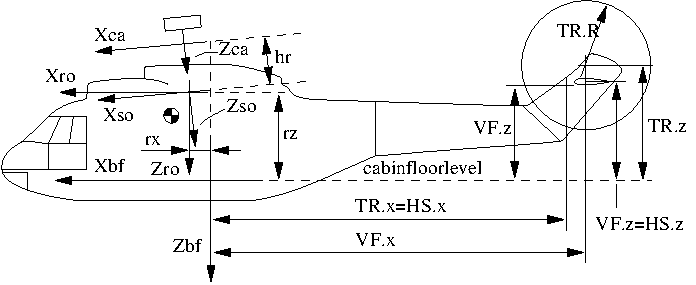
\includegraphics[width=0.7\textwidth]{./figs/chap_introduction/heli_sideview_pdf}
            \else
              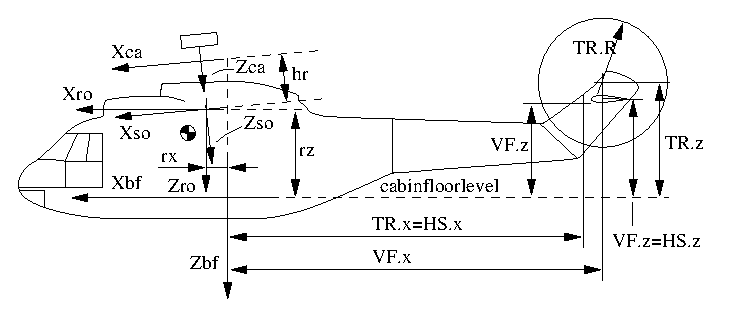
\includegraphics[width=0.7\textwidth]{./figs/chap_introduction/heli_sideview}
            \fi
            \caption[Short caption in the lof: schematic sideview of a helicopter]{Schematic sideview of a helicopter that is by now most likely too long to fit on one line.}
            \label{fig:sideview_reference_frames}
        \end{figure}
        %
%        \begin{figure}[!hbt]
%%             \tiny
%%             \scriptsize
%            \footnotesize
%            \psfrag{Xca}{$\mathsf{X_{hp}}$}
%            \psfrag{Zca}{$\mathsf{Z_{hp}}$}
%            \psfrag{Xro}{$\mathsf{X_{ro}}$}
%            \psfrag{Zro}{$\mathsf{Z_{ro}}$}
%            \psfrag{Xso}{$\mathsf{X_{so}}$}
%            \psfrag{Zso}{$\mathsf{Z_{so}}$}
%            \psfrag{Xbf}{$\mathsf{X_{bf}}$}
%            \psfrag{Zbf}{$\mathsf{Z_{bf}}$}
%            \psfrag{cabinfloorlevel}{$\mathsf{cabin floorlevel}$}
%            \psfrag{TR.R}{$\mathsf{R_{tr}}$}
%            \psfrag{TR.z}{$\mathsf{z_{tr}}$}
%            \psfrag{TR.x=HS.x}{$\mathsf{x_{vf}}$}
%            \psfrag{HS.z}{$\mathsf{z_{hs}}$}
%            \psfrag{VF.z=HS.z}{$\mathsf{z_{hs}}$}
%            \psfrag{VF.z}{$z_{vf}$}
%            \psfrag{VF.x}{$x_{tr} = x_{hs}$}
%            \psfrag{hr}{$h_{r}$}
%            \psfrag{rx}{$r_{x}$}
%            \psfrag{rz}{$r_{z}$}
%            \centering
%            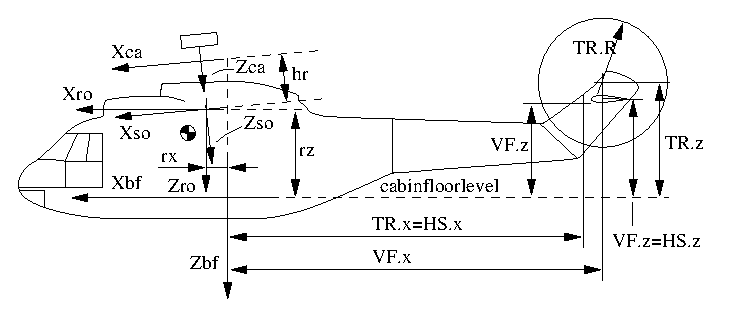
\includegraphics[width=0.7\textwidth]{./figs/chap_introduction/heli_sideview}
%            \caption{Schematic sideview of a helicopter (2)}
%            \label{fig:sideview_reference_frames_2}
%        \end{figure}
        %
        And a fancy figure to show you what is possible with graphics in \LaTeX, see Figure~\ref{fig:blade_geometry}.
        %
%        \begin{figure}[!htb]
%            \centering
%            \subfloat[Equal annuli segment distribution]{%
%                \begin{pspicture}(-0.25,-0.25)(13.125,1.2)
%                    % \psgrid[subgriddiv=1,griddots=10,gridlabels=7pt]
%                    \psdot*[dotsize=4pt](0,0)
%                    % quarter chord line
%                    \psline{-}(-0.25,0)(13.125,0)
%                    % vertical line through centre of rotation
%                    \psline{-}(0,-0.25)(0,0.25)
%                    % blade contours
%                    \pspolygon(3.0625,-0.2363)(13.125,-0.2363)(13.125,0.7088)(3.0625,0.7088)
%                    % blade segment sides
%                    \psline(5.0663,  -0.2363)( 5.0663,  0.7088)
%                    \psline(6.4775,  -0.2363)( 6.4775,  0.7088)
%                    \psline(7.6318,  -0.2363)( 7.6318,  0.7088)
%                    \psline(8.6333,  -0.2363)( 8.6333,  0.7088)
%                    \psline(9.5302,  -0.2363)( 9.5302,  0.7088)
%                    \psline(10.3495, -0.2363)( 10.3495, 0.7088)
%                    \psline(11.1085, -0.2363)( 11.1085, 0.7088)
%                    \psline(11.8190, -0.2363)( 11.8190, 0.7088)
%                    \psline(12.4891, -0.2363)( 12.4891, 0.7088)
%                    % control points
%                    \psdots*[dotsize=4pt](4.0644,  0.0)(5.7719,  0.0)(7.0546,  0.0)(8.1325,  0.0)(9.0817,  0.0)(9.9398,  0.0)(10.7290, 0.0)(11.4637, 0.0)(12.1540, 0.0)(12.8070, 0.0)
%                \end{pspicture}\label{subfig:equal_anulli_distribution}}\\
%            \subfloat[Constant width segment distribution]{%
%                \begin{pspicture}(-0.25,-0.25)(13.125,1.2)
%                    % \psgrid[subgriddiv=1,griddots=10,gridlabels=7pt]
%                    \psdot*[dotsize=4pt](0,0)
%                    % quarter chord line
%                    \psline{-}(-0.25,0)(13.125,0)
%                    % vertical line through centre of rotation
%                    \psline{-}(0,-0.25)(0,0.25)
%                    % blade contours
%                    \pspolygon(3.0625,-0.2363)(13.125,-0.2363)(13.125,0.7088)(3.0625,0.7088)
%                    % blade segment sides
%                    \psline(3.0625,  -0.2363)( 3.0625,  0.7088)
%                    \psline(4.0688,  -0.2363)( 4.0688,  0.7088)
%                    \psline(5.0750,  -0.2363)( 5.0750,  0.7088)
%                    \psline(6.0813,  -0.2363)( 6.0813,  0.7088)
%                    \psline(7.0875,  -0.2363)( 7.0875,  0.7088)
%                    \psline(8.0938,  -0.2363)( 8.0938, 0.7088)
%                    \psline(9.1000,  -0.2363)( 9.1000,  0.7088)
%                    \psline(10.1063, -0.2363)( 10.1063, 0.7088)
%                    \psline(11.1125, -0.2363)( 11.1125, 0.7088)
%                    \psline(12.1188, -0.2363)( 12.1188, 0.7088)
%                    \psline(13.1250, -0.2363)( 13.1250, 0.7088)
%                    % control points
%                    \psdots*[dotsize=4pt](3.5656,  0.00)(4.5719,  0.00)(5.5781,  0.00)(6.5844,  0.00)(7.5906,  0.00)(8.5969,  0.00)(9.6031,  0.00)(10.6094, 0.00)(11.6156, 0.00)(12.6219, 0.00)
%                \end{pspicture}\label{subfig:constant_width_distribution}}
%            \caption[Geometry for a helicopter main rotor blade]{Geometry and segment distributions for a helicopter main rotor blade with 10 segments} \label{fig:blade_geometry}
%        \end{figure}
        %
    \subsection{Alternatives}%
        %
        An alternative to saving figures as PostScript is saving them as PDF. Then, you have to use \emph{pdflatex} which skips the intermediate files. Please note that I will not provide support if you run into problems when you decide to do it this way.
        
        
